\documentclass[a4paper, 11pt]{article}
\usepackage[margin=3cm]{geometry}
\usepackage[]{fontenc}
\usepackage[utf8]{inputenc}
\usepackage[italian]{babel}
\usepackage{geometry}
\geometry{a4paper, top=2cm, bottom=3cm, left=1.5cm, right=1.5cm, heightrounded, bindingoffset=5mm}
\usepackage{amsmath}
\usepackage{amssymb}
\usepackage{gensymb}
\usepackage{graphicx}
\graphicspath{ {./images/} }
\usepackage{psfrag,amsmath,amsfonts,verbatim}
\usepackage{xcolor}
\usepackage{color,soul}
\usepackage{fancyhdr}
\usepackage{indentfirst}
\usepackage{graphicx}
\usepackage{newlfont}
\usepackage{amssymb}
\usepackage{amsmath}
\usepackage{latexsym}
\usepackage{amsthm}
%\usepackage{subfigure}
\usepackage{subcaption}
\usepackage{psfrag}
\usepackage{footnote}
\usepackage{graphics}      
\usepackage{color}
\usepackage{hyperref}
\usepackage{tikz}


\usetikzlibrary{snakes}
\usetikzlibrary{positioning}
\usetikzlibrary{shapes,arrows}

	
	\tikzstyle{block} = [draw, fill=white, rectangle, 
	minimum height=3em, minimum width=6em]
	\tikzstyle{sum} = [draw, fill=white, circle, node distance=1cm]
	\tikzstyle{input} = [coordinate]
	\tikzstyle{output} = [coordinate]
	\tikzstyle{pinstyle} = [pin edge={to-,thin,black}]

\newcommand{\courseacronym}{CAT}
\newcommand{\coursename}{Controlli Automatici - T}
\newcommand{\tipology}{c }
\newcommand{\trace}{3}
\newcommand{\projectname}{Controllo di un rotore con deformazione}
\newcommand{\group}{Z}

%opening
\title{ \vspace{-1in}
		\huge \strut \coursename \strut 
		\\
		\Large  \strut Progetto Tipologia \tipology - Traccia \trace 
		\\
		\Large  \strut \projectname\strut
		\\
		\Large  \strut Gruppo \group\strut
		\vspace{-0.4cm}
}
\author{Autori, \dots}
\date{}

\begin{document}

\maketitle
\vspace{-0.5cm}

Il progetto riguarda il controllo di un rotore ad asse orizzontale con posizione angolare $ \theta (t)$ e velocità angolare $\omega (t)$ rispetto
all’asse del rotore, la cui dinamica viene descritta dalla seguente equazione differenziale 
%
\begin{subequations}\label{eq:system}
\begin{align}
	(m_i e_i^2+I_e) \dot \omega = - \beta \omega - g m_i e_i sin(\theta) + \tau,
\end{align}
\end{subequations}
%
dove la variabile d'ingresso $\tau (t)$ rappresenta la coppia angolare applicata al rotore, il termine $-\beta \omega$ modella l'attrito dell'aria, con $\beta \in \Bbb R$. Il termine $- g m_i e_i sin(\theta)$, dove $g \in \Bbb R$ rappresenta l'accelerazione gravitazionale, modella l'effetto di una deformazione di massa $m_i \in 
\Bbb R $ posta ad una distanza $e_i \in \Bbb R $ dall'asse di rotazione. Infine, il parametro $I_e \in \Bbb R$ rappresenta il momento di inerzia del rotore senza deformazione. Si suppone di poter misurare la posizione angolare $\theta (t)$.


\section{Espressione del sistema in forma di stato e calcolo del sistema linearizzato intorno ad una coppia di equilibrio}

Innanzitutto, esprimiamo il sistema~\eqref{eq:system} nella seguente forma di stato
%
\begin{subequations}
\begin{align}\label{eq:state_form}
	\dot{x} &= f(x,u)
	\\
	y &= h(x,u).
\end{align}
\end{subequations}
%
Pertanto, andiamo a individuare lo stato $x$, l'ingresso $u$ e l'uscita $y$ del sistema come segue 
%
\begin{align*}
	x := \begin{bmatrix} 
                x_1
                \\ 
                x_2
                \end{bmatrix} &:= 
                \begin{bmatrix} 
                \theta 
                \\ 
                \omega
                \end{bmatrix}, \ \
                u := \tau, \ \ y := \theta 
\end{align*}
%
Coerentemente con questa scelta, ricaviamo dal sistema~\eqref{eq:system} la seguente espressione per le funzioni $f$ ed $h$
%
\begin{align*}
	f(x,u) &:= \begin{bmatrix} f_1(x,u)
                \\ 
                f_2(x,u)
                \end{bmatrix} := 
                \begin{bmatrix} 
                x_2 
                \\ 
                \frac{-\beta x_2-g m_i e_i sin(x_1)+ u}{m_i e_i^2 + I_e} 
                \end{bmatrix}
    \\
    h(x,u) &:= x_1
\end{align*}
%
Una volta calcolate $f$ ed $h$ esprimiamo~\eqref{eq:system} nella seguente forma di stato
%
\begin{subequations}\label{eq:our_system_state_form}
\begin{align}
	\begin{bmatrix} 
        \dot x_1
        \\ 
        \dot x_2
        \end{bmatrix} &= 
        \begin{bmatrix} 
        x_2 
        \\ 
        \frac{-\beta x_2-g m_i e_i sin(x_1)+ u}{m_i e_i^2 + I_e} 
        \end{bmatrix}
        \\
        y &= x_1
\end{align}
\end{subequations}
%
Per trovare la coppia di equilibrio $(x_e, u_e)$ di~\eqref{eq:our_system_state_form}, andiamo a risolvere il seguente sistema di equazioni
%
\begin{align}
	\begin{bmatrix} 
        0
        \\
        0
        \end{bmatrix} = 
        \begin{bmatrix}
        x_2
        \\ 
        \frac{-\beta x_2-g m_i e_i sin(x_1)+ u}{m_i e_i^2 + I_e} 
        \end{bmatrix} ,
\end{align}
%
dal quale otteniamo
%
\begin{align}
	x_e := \begin{bmatrix} x_{1e}
                \\ 
                x_{2e}
                \end{bmatrix} :=
                \begin{bmatrix} 
                \theta_e 
                \\ 
                0
                \end{bmatrix}, \ \
u_e:= \frac{g m_i e_i}{2}.\label{eq:equilibirum_pair}
\end{align}
%
Definiamo le variabili alle variazioni $\delta x$, $\delta u$ e $\delta y$ come 
%
\begin{align*}
	\delta x &= x - x_e, 
	\quad
	\delta u = u - u_e, 
	\quad
	\delta y = y - y_e.
\end{align*}
%
L'evoluzione del sistema espressa nelle variabili alle variazioni pu\`o essere approssimativamente descritta mediante il seguente sistema lineare
%
\begin{subequations}\label{eq:linearized_system}
\begin{align}
	\delta \dot{x} &= A\delta x + B\delta u
	\\
	\delta y &= C\delta x + D\delta u,
\end{align}
\end{subequations}
%
dove le matrici $A$, $B$, $C$ e $D$ vengono calcolate come
%
\begin{subequations}\label{eq:matrices}
\begin{align}
	A &= \begin{bmatrix}
	    \frac{\partial f_1(x,u)}{\partial x_1} & \frac{\partial f_1(x,u)}{\partial x_2} 
        \\ 
        \frac{\partial f_2(x,u)}{\partial x_1} & \frac{\partial f_2(x,u)}{\partial x_2} 
        \end{bmatrix}_{\substack{x=x_e \\ u = u_e}}
        &= \begin{bmatrix}
            0 & 1 
            \\ 
            \frac{-g m_i e_i cos(x_1)}{m_i e_i^2 + I_e} & \frac{\beta}{m_i e_i^2 + I_e}
        \end{bmatrix}_{\substack{x_1=\frac{\pi}{6} \\ x_2=0 \\  u=u_e}}
        &= \begin{bmatrix}
            0 & 1 
            \\ 
            \frac{-g m_i e_i \sqrt{3}}{2(m_i e_i^2 + I_e)} & \frac{\beta}{m_i e_i^2 + I_e}
        \end{bmatrix}
	\\
	B &= \begin{bmatrix} 
            \frac{\partial f_1(x,u)}{\partial u}
            \\ 
            \frac{\partial f_2(x,u)}{\partial u} \end{bmatrix}_{\substack{x=x_e \\ u=u_e}}
= \begin{bmatrix} 0 \\ \frac{1}{m_i e_i^2 + I_e} \end{bmatrix}
	\\
	C &= \begin{bmatrix} 
            \frac{\partial h(x,u)}{\partial x_1} & \frac{\partial h(x,u)}{\partial x_2} \end{bmatrix}_{\substack{x=x_e \\  u=u_e}}
=\begin{bmatrix} 1 & 0 \end{bmatrix}
	\\
	D &= \begin{bmatrix} \frac{\partial h(x,u)}{\partial u} \end{bmatrix}_{\substack{x=x_e \\ u=u_e}}
= 0
\end{align}
\end{subequations}
%
\section{Calcolo Funzione di Trasferimento}

In questa sezione, andiamo a calcolare la funzione di trasferimento $G(s)$ dall'ingresso $\delta u$ all'uscita $\delta y$ mediante la seguente formula 
%
%
\begin{align}\label{eq:transfer_function}
G(s) = C(sI_3 - A)^{-1}C +D = \frac{0.01998}{s^2 + 0.999 s + 0.08479}.
\end{align}
%
Dunque il sistema linearizzato~\eqref{eq:linearized_system} è caratterizzato dalla funzione di trasferimento~\eqref{eq:transfer_function} con 2 poli \\ $p_1 = -0.9054$, $p_2 = -0.0936$ e nessuno zero. In Figura \ref{fig:bode1} mostriamo il corrispondente diagramma di Bode. 

\begin{figure}[h]
\centering
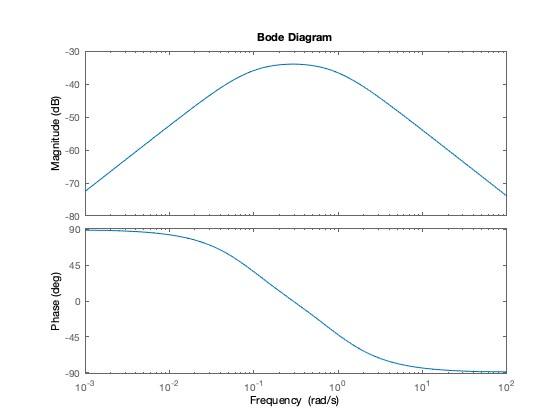
\includegraphics[width=0.5\textwidth]{fig_bode_G(s).jpg}
\caption{Diagramma di Bode della funzione di trasferimento $G(s)$}
\label{fig:bode1}
\end{figure}

\section{Mappatura specifiche del regolatore}
\label{sec:specifications}

Le specifiche da soddisfare sono
\begin{itemize}
	\item[1)] Errore a regime $|e_{\infty}| \leq e^{\star} = 0.01$ in risposta a un gradino $w(t) = \frac{\pi}{6} \cdot 
 1(t) $ e $d(t)=  \frac{\pi}{6} \cdot 1(t)$ \\
	\item[2)] Margine di fase $M_f \geq 45^{\degree}$.\\
    \item[3)] Sovraelongazione percentuale massima del 5\%: $S \% \leq 5\% $ .\\
    \item[4)] Il tempo di assestamento all' $\epsilon \% = 5 \% $ deve essere inferiore al valore fissato: $T_{a, \epsilon} = 0.075$s.\\
	\item[5)] Il disturbo sull'uscita $d(t)$, con una banda limitata nel range di pulsazioni [0,0.1], deve essere abbattuto di almeno 50 dB.\\
	\item[6)] Il rumore di misura $n(t)$, con una banda limitata di pulsazioni [$10^3, 10^6$], deve essere abbattuto di almeno 35 dB.
\end{itemize}
%
Andiamo ad effettuare la mappatura punto per punto le specifiche richieste. 

%
\begin{subequations}\label{eq:spec}
\begin{align}
\xi &= \frac{\ln(S_p)}{\sqrt{\ln(S_p)^2 + \pi^2}} = \frac{\ln(5)}{\sqrt{\ln(5)^2 + \pi^2}} = 0.4559
\\
M_{f,spec} &= \xi \cdot 100 = 45.59 
\\ 
\omega_{c,min} &= \frac{300}{M_{f,spec} T_{a, \epsilon}} = \frac{300}{45.59 \cdot 0.075} = 87.7290
\end{align}
\end{subequations}
%

Pertanto, in Figura \ref{fig:bode2}, mostriamo il diagramma di Bode della funzione di trasferimento $G(s)$ con le zone proibite emerse dalla mappatura delle specifiche.

\begin{figure}[h]
\centering
\includegraphics[width=0.5\textwidth]{fig_bode_G(s)_spec.jpg}
\caption{Diagramma di Bode della funzione di trasferimento $G(s)$ con specifiche}
\label{fig:bode2}
\end{figure}

Come si può notare dalla figura, la funzione di trasferimento $G(s)$ interseca l'asse 0dB, pertanto il criterio di Bode per la stabilità di un sistema è applicabile.



\section{Sintesi del regolatore statico}
\label{sec:static_regulator}

In questa sezione progettiamo il regolatore statico $R_s(s)$ partendo dalle analisi fatte in sezione~\ref{sec:specifications}.

\dots

Dunque, definiamo la funzione estesa $G_e(s) = R_s(s)G(s)$ e, in Figura \ref{fig:bode3}, mostriamo il suo diagramma di Bode per verificare se e quali zone proibite vengono attraversate.
\dots
\\
Al fine di garantire il rispetto del vincolo 1 abbiamo progettato il regolatore statico nel seguente modo. 
Dalle specifiche sull'errore a regime risulta che il guadagno del regolatore statico $\mu _r $ deve essere maggiore di $\mu^{\star}$. 

%
\begin{subequations}\label{eq:mu_r}
\begin{align}
\mu_r \geq  \mu^{\star} = \frac{D^{\star} + W^{\star}}{e^{\star}}
\end{align}
\end{subequations}
%

Sostituendo otteniamo 
$$
\mu^{\star} = \frac{\frac{\pi}{6} + \frac{\pi}{6}}{0.01} \simeq 104.72
$$
Infine noi abbiamo scelto $\mu_r = 0.3 \cdot 10^4$ per soddisfare il vincolo sull'attenuazione del disturbo. 

\begin{figure}[h]
\centering
\includegraphics[width=0.5\textwidth]{fig_bode_Ge(s).jpg}
\caption{Diagramma di Bode della funzione di trasferimento $G_s(s)$}
\label{fig:bode3}
\end{figure}


\section{Sintesi del regolatore dinamico}

In questa sezione, progettiamo il regolatore dinamico $R_d(s)$. 
%
Dalle analisi fatte in Sezione~\ref{sec:static_regulator}, notiamo di essere nello Scenario di tipo B. Dunque, progettiamo $R_d(s)$ ricorrendo a una rete anticipatrice.
%
\begin{subequations}\label{eq:reg_dinamico}
\begin{align}
R_d(s) = \frac{1 + \tau s}{(1 + \alpha \tau s)(1 + \frac{1}{4 \cdot 10^2}s)}
\end{align}
\end{subequations}
%
Con 
$$
\tau = \frac{M^{\star} - cos(\varphi^{\star})}{\omega_c^{\star} sin(\varphi^{\star})}
$$
e 
$$
\alpha \tau = \frac{cos(\varphi^{\star}) - \frac{1}{M^{\star}}}{\omega_c^{\star} sin(\varphi^{\star})}
$$


In Figura \ref{fig:L_s}, mostriamo il diagramma di Bode della funzione d'anello $L(s) = R_d(s) G_e(s)$

\begin{figure}[h]
\centering
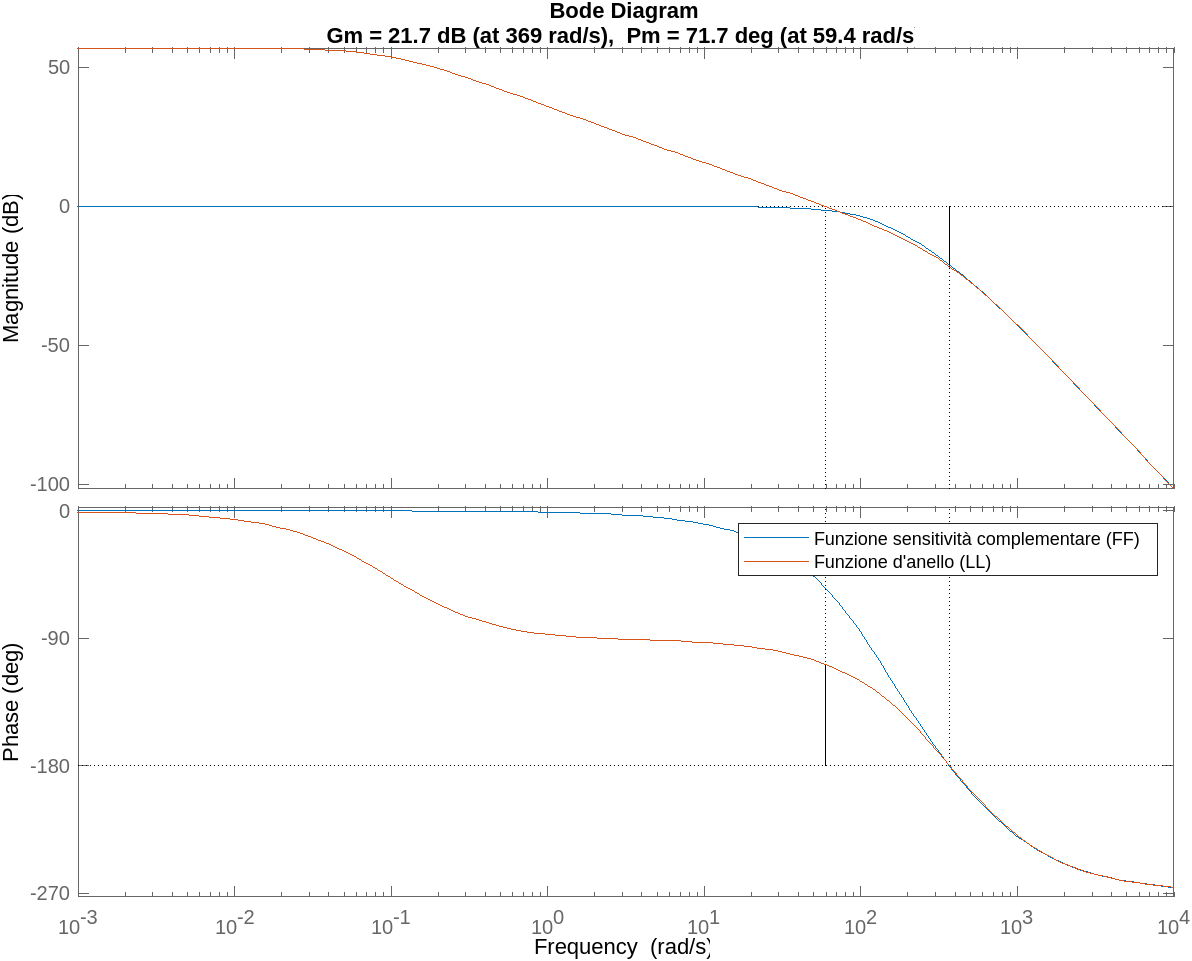
\includegraphics[width=0.5\textwidth]{images/Figure_4.png}
\caption{Diagramma di Bode della funzione $L(s)$}
\label{fig:L_s}
\end{figure}






\section{Test sul sistema linearizzato}

In questa sezione, testiamo l'efficacia del controllore progettato sul sistema linearizzato con $w(t) = 20 \cdot 
 1(t) $, $d(t)= \sum_{k=1}^4 0.1 \cdot \sin(0.025kt)$ e $n(t)= \sum_{k=1}^4 0.6 \cdot \sin(10^3 kt)  $. 
 \\
 In figura \ref{fig:grad1} osserviamo la risposta del sistema ponendo un gradino $ w(t) = 20 \cdot 1(t)$ all'ingresso. 
 

 
\begin{figure}[h]
\centering
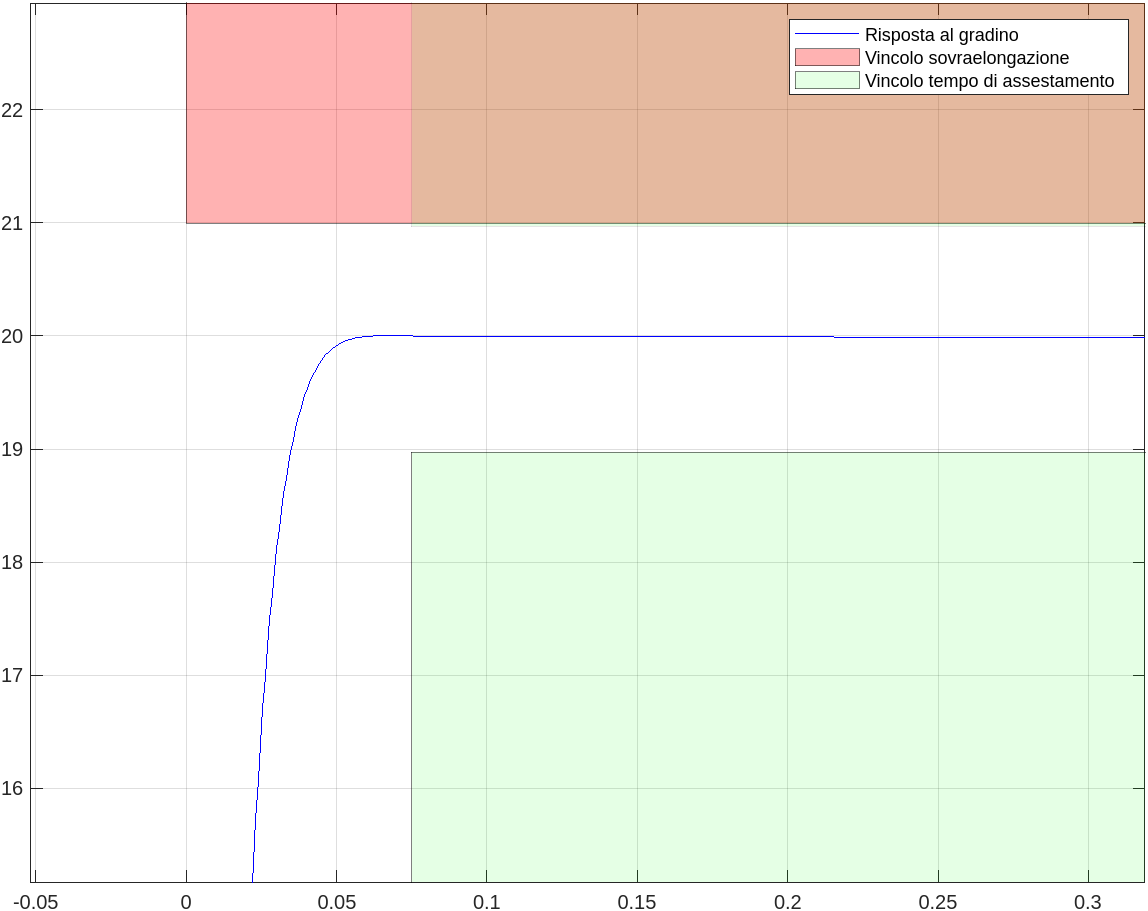
\includegraphics[width=0.5\textwidth]{images/Figure_5.png}
\caption{Risposta al gradino}
\label{fig:grad1}
\end{figure}

Mentre nelle figure \ref{fig:distD} e \ref{fig:distN} osserviamo l'andamento dell'uscita del sistema rispettivamente a fronte di un disturbo $ d(t) $ e $n(t)$. 

\begin{figure}[h]
\centering
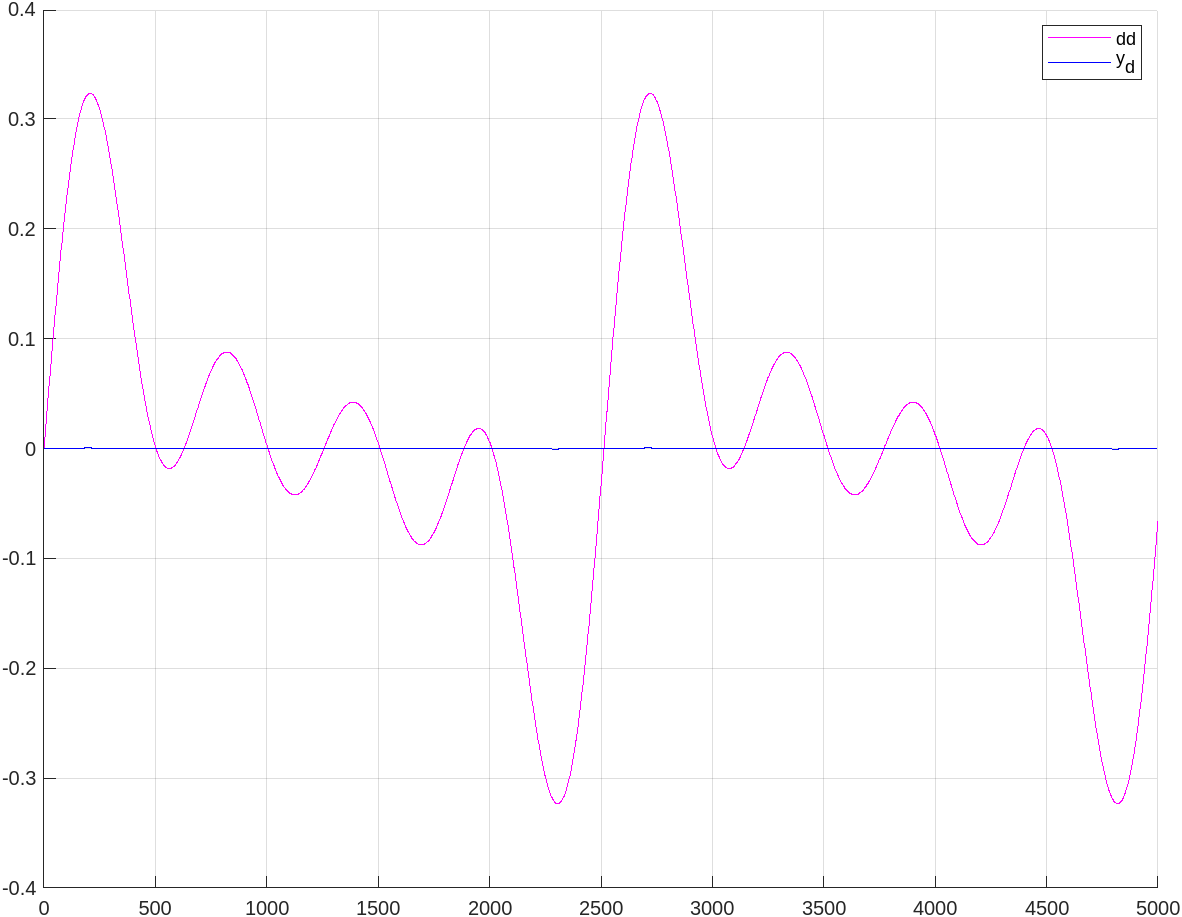
\includegraphics[width=0.5\textwidth]{images/Figure_6.png}
\caption{Attenuazione del disturbo $d(t)$}
\label{fig:distD}
\end{figure}

\begin{figure}[h]
\centering
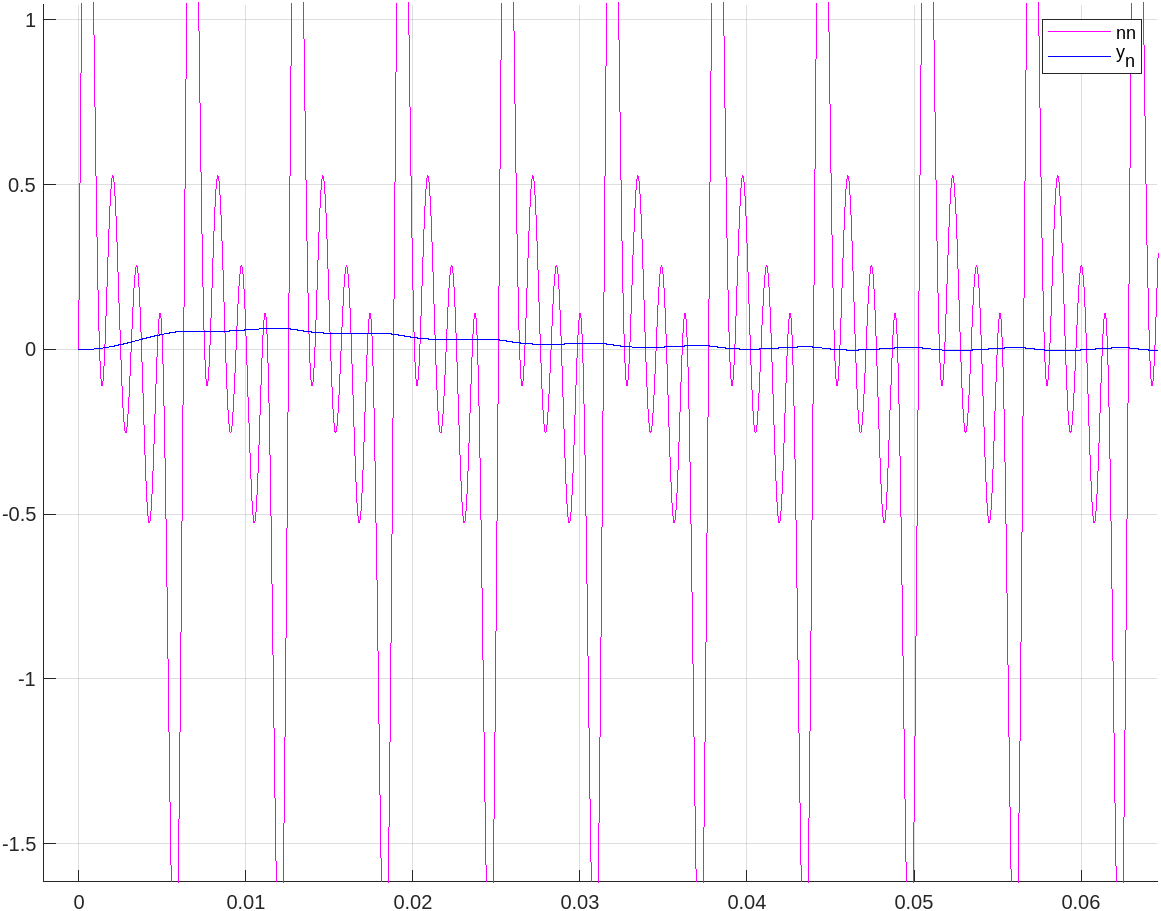
\includegraphics[width=0.5\textwidth]{images/Figure_7.png}
\caption{Attenuazione del disturbo $n(t)$}
\label{fig:distN}
\end{figure}



\section{Test sul sistema non lineare}
In questa sezione, testiamo l'efficacia del controllore progettato sul modello non lineare con $w(t) = 20 \cdot 
 1(t) $, $d(t)= \sum_{k=1}^4 0.1 \cdot \sin(0.025kt)$ e $n(t)= \sum_{k=1}^4 0.6 \cdot \sin(10^3 kt)  $.

 Per testarne l'efficacia, utilizziamo Simulink. Per farlo creiamo un modello per il disturbo $n(t)$, uno per il disturbo $d(t)$ e uno per il sistema non lineare, ottenuto tramite combinazione di blocchi somma, gain e integratore (nel quale è possibile definire le condizioni iniziali del sistema). Infine, colleghiamo i vari modelli creati insieme al blocco del regolatore (definito dalla sua funzione di trasferimento) e simuliamo il sistema con un ingresso gradino. In Figura x si mostra l'uscita del sistema risultante
\begin{figure}[h]
\centering
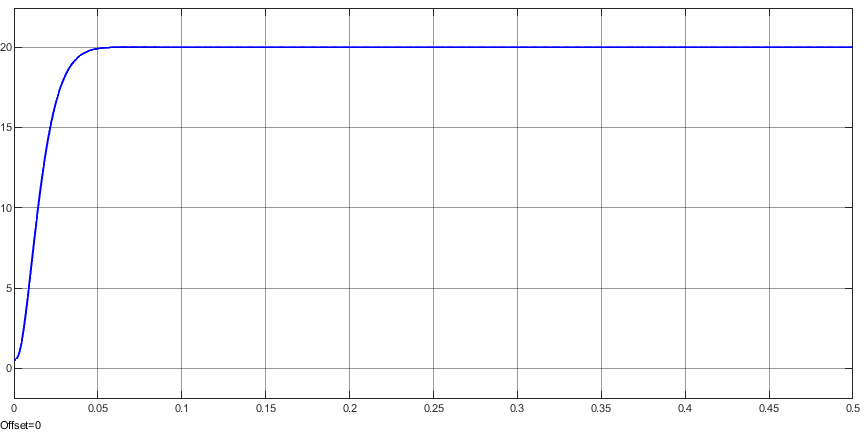
\includegraphics[width=0.5\textwidth]{images/test_non_lineare.png}
\caption{Uscita del sistema non linearizzato}
\label{fig:test_non_lineare}
\end{figure}

\section{Punti opzionali}

\subsection{Primo punto}

L'animazione della pala è stata creata partendo dall'oggetto "antenna.Polygon" che permette di creare un poligono su un piano X-Y e di farlo ruotare attorno al proprio asse. Per la durata dell'intervallo di integrazione, calcolando la posizione in alcuni istanti di tempo è stato possibile ruotare il poligono di quell'angolo e dunque di simulare la rotazione del rotore attorno all'asse Z.


\subsection{Secondo punto}

\dots

\subsection{Terzo punto}

\dots

\section{Conclusioni}

\dots

\end{document}
